\chapter{The state space structure of Spiral Defect Chaos}\label{sec:chap4}

The co-existence of ideal straight rolls (ISRs) and spiral-defect chaos (SDC) as bistable states in Rayleigh-B\'{e}nard convection above the onset of the linear instability is well established in extended spatial domains ($\Gamma \ge 40$ where $\Gamma$ is the aspect ratio of the domain). However, multiple stable states have also been found independently, raising questions about the precise understanding of this observed bistability in extended domains. In this study, we isolate the localised structures of SDC by gradually reducing the spatial domain. By minimising the domain systematically to $\Gamma = 2\pi$, SDC appears transiently and eventually stabilises into new stable states referred to as elementary states. These elementary states are visibly and statistically similar to the spatially local patterns of SDC, indicative of invariant solutions underpinning the pattern formation in SDC.

To understand the state space structure further, we have examined the edge between ISRs and the elementary states, revealing multiple edge states, and conducted a series of numerical simulations along the unstable manifolds of unstable ISRs. The unstable ISRs near the Busse balloon are connected to stable ISRs and the base state through networks of heteroclinic orbits, forming a basin of attraction for each stable ISR. In contrast, the unstable ISRs further from the Busse balloon contain some unstable manifolds, along which the solution trajectory leads to SDC, suggesting that these unstable ISRs sit on the boundary between stable ISRs and SDC. Finally, we propose a state-space structure around the basic heat conduction state, stable/unstable ISRs, elementary states and transient SDC.

% \section{Introduction}\label{sec:rbc_intro}
% 
% Rayleigh-B\'{e}nard convection (RBC) concerns the fluid motion confined between two parallel walls, separated by a distance $d$, heated from below. The motion of the fluid is effectively driven by unstable stratification due to temperature gradients ($\Delta T/d$) across the walls. Given a large enough temperature gradient, a non-trivial fluid motion occurs, often developing into a spatially varying structure known as a convection pattern. This motion is described in terms of the Rayleigh number $Ra = \alpha g d^3 \Delta T / \nu \kappa$, Prandtl number $Pr = \nu / \kappa$ and aspect ratio of the experimental/computational domain $\Gamma = L/d$, where $\alpha, g, \Delta T, \nu, \kappa, L$ refers to the thermal expansion coefficient, acceleration due to gravity, temperature difference between the bottom and top wall, kinematic viscosity thermal diffusivity, domain's length and span respectively. An important question that underpins RBC is often as follows: Given the Rayleigh number ($Ra$), Prandtl number ($Pr$) and aspect ratio ($\Gamma$) of a fluid system, what convection pattern arises and what is its associated heat flux? 
% 
% \subsection{Multiple convection states}\label{sec:rbc_mulstate}
% 
% While the Busse balloon describes the stability of ISRs over a continuum of wavenumbers (at given ${Ra}$ and ${Pr}$), predicting the wavenumber of an ISR state remains an ongoing challenge \cite{bodenschatz2000}. Experimental investigations of RBC in moderate domains ($\Gamma \geq 7$) showed that ISRs in rectangular (straight rolls) and cylindrical (concentric rolls) domains are stable. Consider $\varepsilon (\equiv (Ra-Ra_c)/Ra_c$, where $Ra_c$ is the critical $Ra$ for the onset of linear instability for ISRs) as a control parameter referred to as the reduced Rayleigh number. As $\varepsilon$ is increased continuously from below the onset, the initial ISRs become unstable and transform into another set of ISRs with a different wavelength. With the marginal increase of $\varepsilon$, this process is repeated and the ISRs undergo hysteretic transverse wavelength adjustments, adhering to the stability boundaries of the Busse balloon \cite{steinberg1985,croquette1989a}. When ISRs become unstable, roll dislocations and defects can be nucleated near the boundary or bulk, modifying the effective roll wavenumber as they travel through the domain \cite{croquette1989a}. This observation implies that the wavenumber of an ISR state depends on the state's history or the system's initial condition \cite{bodenschatz2000}.
% 
% It is worth noting that the solutions in the form of ISRs appear to be an exception rather than the rule \cite{croquette1989b}. The coexistence of multiple `non-ISR' states, in the form of squares, travelling/stationary targets, giant rotating spirals, and oscillatory convection patterns have been found over several years \cite{legal1985, croquette1989a, plapp1998, hof1999, rudiger2000, boronska2010a}. Investigation of cylindrical RBC with small aspect-ratio ($\Gamma = 2$) revealed eight stationary states (at the same ${Ra} = 142000$), and two oscillatory states ($Ra > 14200$) \cite{hof1999}. These findings were later supported by numerical experiments and bifurcation analyses \cite{ma2006, boronska2010a, boronska2010b}. In particular, bifurcation analyses performed by \cite{ma2006}, revealed twelve stable branches in the form of symmetric and asymmetric convection rolls near onset ($Ra \leq 2500$), with the potential emergence of hundreds of branches at higher Rayleigh numbers, ${Ra} \leq 30000$ \cite{boronska2010b}. In larger domains ($\Gamma \geq 28$), giant rotating spirals were identified and thoroughly investigated \cite{plapp1996, plapp1998}. Experimental and numerical studies of RBC with varying sidewall boundary conditions (i.e. thermally insulating, conducting and no-slip) \cite{tuckerman1988, siggers2003, paul2003, boulle2022}, non-Boussinesq convection \cite{bodenschatz1991, bodenschatz1992}, and rotational effects \cite{hu1997} were investigated, where multiple states were also reported. More recently, \cite{Reetz2020part1, Reetz2020part2} computed up to sixteen stable and unstable invariant states and identified heteroclinic orbits between the multiple states in an inclined RBC.
% 
% \subsection{Spiral defect chaos}\label{sec:rbc_sdc}
% Convection rolls exhibiting spatio-temporal chaotic behaviour known as spiral defect chaos (SDC) are found in the same parameter space of $\varepsilon$, where ISRs were expected \cite{Morris93, hu1993, Decker94, hu1995a,hu1995b, morris1996, Cakmur97, ahlers1998, egolf1998, chiam2003, vitral2020}. It is well established that SDC exists as an intrinsic state of RBC, independent of sidewall conditions \cite{morris1996}. SDC has also been found in numerical simulations of the two-dimensional Swift-Hohenberg equations \cite{swift1977, xi1993, xi1995, schmitz2002, karimi2011}. Some investigations into quantifying the onset of SDC in terms of Rayleigh number remain inconclusive. The critical reduced Rayleigh number for the onset of SDC, $\varepsilon_s$, has been observed to decrease with increasing $\Gamma$, and increase with increasing $Pr$ \cite{hu1995a, hu1995b, bajaj1997, Cakmur97, bodenschatz2000}. It is worth noting that SDC has been reported in larger domains ($\Gamma \geq 20$) only, implying that there exists a minimal $\Gamma$ for SDC to occur \cite{bodenschatz2000}, further supporting the dependence of $\varepsilon_s$ on $\Gamma$ mentioned above. This is also consistent with the leading Lyapunov exponents, which become smaller with decreasing aspect ratios, $\Gamma$, albeit at larger $\varepsilon = 2.5$ \cite{egolf2000, paul2007}. Investigations into the spatial-temporal characteristics of SDC, such as the quantification of the averaged roll-curvature \cite{hu1995a, hu1995b}, probability of spirals \cite{ecke1995,liu1996} and correlation length-/time-scales \cite{Morris93,morris1996,Cakmur97} have been studied. Specifically, the correlation length-scales \cite{Morris93, morris1996, Cakmur97} of SDC appear to scale exponentially as $\varepsilon$ is increased. Furthermore, spatio-temporal chaotic behaviour reminiscent to SDC has been found in other pattern-formation systems such as rotational RBC \cite{hu1997}, dielectric barrier discharge \cite{dong2005} and chemical systems \cite{affan2014}.
% 
% Given the co-existence of ISRs and SDC in the parameter space of $\varepsilon$, it is known that they form bistability at $Pr \approx 1$ in a spatially extended domain, supported by experiments over a range of $\varepsilon(>0)$ \cite{Cakmur97}. Only carefully prepared experiment setups led to ISRs while most initial conditions yield SDC. In other words, the asymptotic state of RBC depends on its initial conditions, reminiscent of the hysteretic behaviour of RBC discussed in \S\ref{sec:rbc_mulstate}. The chaotic state of SDC is unstable at $Pr=4$, where multiple spiral patterns coarsen into a single spiral, before evolving into straight-curved rolls over a long period \cite{bajaj1997}. This implies that the behaviour of SDC depends on $Pr$.

\section{Objectives}\label{sec:rbc_objs}
The bistability between SDC and ISR is well established, but this also opens a question of how it is connected with the previous findings of multiple stable states (see \S \ref{sec:bkgrd_RBC}).
It is worth noting that a possible parameter in exploring this connection appears to be the domain size.
Bistability has been reported in domains much larger ($\Gamma = 50$) than the multiple states found in small-to-moderate domains ($\Gamma \leq 10$) \cite{cakmur_bistability_1997}.
Furthermore, giant rotating spirals have been found in domains comparable to the horizontal length scale of SDC \cite{plapp_core_1996, plapp_dynamics_1998}. 
Under this premise, the scope of this study is to explore how SDC, ISRs and multiple states are organised within a state space, where stable/unstable equilibria and their manifolds (or linear stability) could provide useful physical insights into the state transition dynamics. 

Motivated by the observation that SDC consists of several localised structures that resemble multiple states (i.e. travelling waves, spirals, asymmetric states), we first seek to isolate these states by minimising the domain systematically.
Confined within the minimal domain, SDC is found to appear only transiently and does not sustain for a long time.
The transient SDC state eventually stabilises into a large number of stable multiple states, which will be referred to as the `elementary' states of SDC, and they are subsequently found within the minimal domain.
As we shall see later, these elementary states remarkably resemble local structures of SDC observed in wide computational domains, indicating that they possibly underpin the formation of SDC.
Next, the state-space boundaries between SDC and ISRs are explored by employing the edge-tracking technique \cite{skufca_edge_2006,schneider_turbulence_2007}, unveiling the existence of multiple edge states sitting on the boundaries.
Finally, to understand the role of the unstable ISRs outside the Busse balloon, we perform a series of numerical experiments, in which a small perturbation is added along the unstable manifolds of several (unstable) ISRs outside of the Busse balloon.
We shall see that some of their unstable manifolds are connected to stable ISRs within the Busse balloon, while the others are linked to transient SDC, which is subsequently stabilised into an elementary state.
This suggests that some of the unstable ISRs act as signposts for the state-space boundary between stable ISRs and SDC (and/or elementary states). 

The main contributions of the present chapter can be briefly summarised as follows,
\begin{enumerate}
    \item Discovery of a number of stable invariant solutions which underpin the localised structures of SDC by minimising the computational domain for SDC (sectisn \ref{sec:rbc_mindom});
    \item Computation of some of multiple `edge states' sitting on the separatrix between SDC and ISRs (section \ref{sec:rbc_edgestate});
    \item Several heteroclinic orbits connecting unstable ISRs and stable ISRs near the boundaries of the Busse balloon (section \ref{sec:rbc_heteroclinic});
    \item The role of unstable ISRs far from the Busse balloon acting as a signpost between ISRs and SDC (section \ref{sec:rbc_chaoticsaddle}).
\end{enumerate}

\section{Problem formulation}\label{sec:rbc_2}
\subsection{Rayleigh-Benard convection (RBC)}
The motion of fluid flow in an RBC system (see \S \ref{sec:bkgrd_overview}), is govern by the non-dimensionalised Navier-Stokes equations with Boussinesq approximation,
% We consider a buoyancy-driven flow of an incompressible fluid separated by a vertical height of $d$, confined between an upper wall of uniform temperature $T_U$, and a lower wall of uniform temperature $T_L$. The temperature of the lower wall is higher than the temperature of the upper wall ($\Delta T = T_L - T_U > 0$) such that the fluid is unstably stratified. The fluid has a density of $\rho$, a thermal diffusivity of $\kappa$, and a kinematic viscosity of $\nu$.  The non-dimensionalised governing equations with the Boussinesq approximation for buoyancy-driven flows are given by
\begin{subequations}\label{eq:rbc_rbc}
\begin{equation}
    \frac{\partial \mathbf{u}}{\partial t} + (\mathbf{u} \cdot \nabla) \mathbf{u} = -\nabla p + Pr\nabla^2 \mathbf{u} + RaPr\theta \mathbf{{j}},
\end{equation}
\begin{equation}
    \frac{\partial \theta}{\partial t} + (\mathbf{u} \cdot \nabla) \theta = \nabla^2 \theta,
\end{equation}
\begin{equation}
    \nabla \cdot \mathbf{u} = 0,
\end{equation}
\end{subequations}
with the following boundary conditions at the wall,
\begin{subequations}\label{eq:rbc_bc}
\begin{equation}
    \mathbf{u}|_{y=0,1} = 0, \quad \theta|_{y=0} = 1, \quad \theta|_{y=1} = 0, 
\end{equation}
\end{subequations}
and the periodic boundary condition in the horizontal direction.
Here, $t$ denotes the time scaled by the vertical thermal diffusion time, $d^2/\kappa$, and $\mathbf{x}(=(x,y,z))$ is the spatial coordinates non-dimensionalised by $d$, where $x$ and $z$ are two orthogonal horizontal directions and $y$ is the vertical direction.
$\mathbf{u}(=(u,v,w))$ is the velocity vector scaled with $\kappa/d$, $p$ the pressure scaled with $ \rho \kappa^2 / d^2 $, $\theta(\equiv(T-T_U)/\Delta T)$ the non-dimensional temperature with $T$ being the absolute temperature, and $\mathbf{j}$ denotes the unit vector in $y$-direction. 
The Rayleigh number and the Prandtl numbers are defined as in \S\ref{sec:bkgrd_overview}: $Ra = \alpha g d^3 \Delta T / \nu \kappa$, Prandtl number $Pr = \nu / \kappa$. Throughout this study, $Pr=1$ is set. 

\subsection{Numerical method}
The governing equations are solved numerically using Nektar++, an open-source spectral/\emph{hp}-element method framework \cite{cantwell_nektar_2015, moxey_nektar_2020}.
An initial computational mesh, composed of quadrilateral elements, in the $x$-$y$ plane is generated using Gmsh \cite{geuzaine_gmsh_2009} and then refined by Nekmesh, the mesh generator available in Nektar++.
Several computational domains of different sizes are prepared: $(L_x, L_y, L_z) = (32\pi, 1, 32\pi), (16\pi, 1, 16\pi), (8\pi, 1, 8\pi)$, $(4\pi, 1, 4\pi)$.
The spatial domain is discretised using a quasi-3D approach with spectral/\emph{hp} elements in $x$-$y$ domain and Fourier expansions in $z$-direction.
The discretised equations are subsequently solved using a velocity-correction method based on a second-order implicit-explicit temporal scheme (see \S \ref{sec:nm_vcs}).
Since different computational domain sizes were considered, the spatial distribution of spectral/\emph{hp} elements in the $x$-$y$ plane and Fourier expansions along $z$ was kept constant.
A spatial resolution of $(\Delta x, \Delta y|_{y=0,d}, \Delta y|_{y={d/2}}, \Delta z) = (0.1\pi, 0.0549, 0.367, 0.25\pi)$ with polynomial order $P=4$, and temporal resolution of $\Delta t = 0.0125$ was sufficient to establish numerical independence -- for example, the Nusselt number, $Nu(=-\int_{x,z}\frac{\partial \theta}{\partial y}|_{y=0} \; \mathrm{d}x\mathrm{d}z)$, varies less than $10^{-5}$ when $P$ was increased to $P=5$.

\subsection{Linear stability analysis of ISRs}\label{sec:rbc_lsa}
As discussed in \S\ref{sec:rbc_objs}, we will perform a set of numerical experiments, in which a small perturbation about several unstable ISRs is added along their unstable manifolds.
To obtain the direction of the unstable manifolds (i.e. linear instability eigenfunctions), we consider a small perturbation about the ISR (base) state: 
\begin{subequations}\label{eq:rbc_basepert}
\begin{equation}
    \mathbf{u}(\mathbf{x}, t) = \mathbf{u}_{ISR,q}(\mathbf{x}) + \mathbf{u'}(\mathbf{x}, t),
\end{equation}
\begin{equation}
    \theta(\mathbf{x}, t) =\theta_{ISR,q}(\mathbf{x})  + \theta'(\mathbf{x}, t), 
\end{equation}
\begin{equation}
    p(\mathbf{x}, t)  = p_{ISR,q}(\mathbf{x})  + p'(\mathbf{x}, t),
\end{equation}
\end{subequations}
where $\mathbf{s}  = [\mathbf{u}, \theta, p]^T$, $\mathbf{s}_{ISR,q}=[\mathbf{u}_{ISR,q}, \theta_{ISR,q}, p_{ISR,q}]^T$ and $\mathbf{s}'=[\mathbf{u}', \theta', p']^T$ refers to solution vector, the ISR (base) state of a given wavenumber, $q$, and the perturbation respectively.
This is rooted in linear stability methods discussed earlier in \S \ref{sec:bkgrd_transitional}, and its numerical technique is presented in \S \ref{sec:nm_arnoldi}.
Substitution of (\ref{eq:rbc_basepert}) into (\ref{eq:rbc_rbc}) leads to the following linearised equations:
\begin{subequations}\label{eq:rbc_linearised}
\begin{equation}
    \frac{\partial \mathbf{s'}}{\partial t} = \mathcal{A}(\mathbf{s}_{ISR,q}; Ra, Pr) \mathbf{s'}, 
\end{equation}
where
\begin{equation}
\mathcal{A}(\mathbf{s}_{ISR,q}; Ra, Pr) =
    \left(
    \begin{array}{c c c}
      - (\mathbf{U} \cdot\nabla) - (\nabla \mathbf{U} \cdot) + Pr\nabla^2 & RaPr\mathbf{\hat{j}} & -\nabla \\
      -(\nabla \Theta \cdot)  &  - (\mathbf{U} \cdot \nabla) + \nabla^2 & 0 \\
      \nabla \cdot  & 0  & 0
    \end{array}
    \right).
\end{equation}
\end{subequations}
For the sake of simplicity here, we will only consider the ISRs invariant along $z$-direction.
Since the ISRs are also assumed periodic in $x$-direction, the following form of normal-mode solution can be considered:
\begin{equation}\label{eq:rbc_ansatz}
    \mathbf{s}' (\mathbf{x},t) = \mathbf{\breve{s}}(x,y)e^{i(\alpha x+\beta z)+\lambda t} + \text{c.c},
\end{equation}
where $\lambda, \alpha$ and $\beta$ are the complex frequency, the streamwise wavenumber (or the Floquet exponent), and the spanwise wavenumber, respectively. Using the periodic nature of $\mathbf{\breve{s}}(x,y)$ in $x$-direction, (\ref{eq:rbc_ansatz}) can also be written as 
\begin{equation}\label{eq:rbc_simAnsatz}
    \mathbf{s}' (\mathbf{x},t) = \left[\sum_{n=-\infty}^{\infty}\mathbf{\breve{\breve{s}}}_n(y)e^{i \frac{2\pi}{L_x}(n+\epsilon) x} \right] e^{i\beta z+\lambda t} + \text{c.c},
\end{equation}
where $\epsilon(=\alpha L_x/(2\pi))$ is the Floquet detuning parameter with $0 \leq \epsilon \leq 1/2$. Since the stability analysis here will be limited to the identification of unstable manifolds of ISRs in a fixed computational domain, $\epsilon=0$ (fundamental mode) is considered only - note that the modes associated with $\epsilon \ne 0$ are only observed in the $x$ domains greater than $L_x$.

Substituting \eqref{eq:rbc_simAnsatz} into (\ref{eq:rbc_linearised}) leads to a discretised eigenvalue problem in terms of the eigenvalue $\lambda$, where the wavenumber in the $z$-direction must be restricted to be $\beta=2 \pi m/L_z$, and $m$ is a positive integer, for the given computational domain. The resulting eigenvalue problems are solved using a time-stepper-based iterative Arnoldi algorithm \cite{tuckerman2000}, implemented in Nektar++, which has been verified in various applications \cite{cantwell2015}. The eigenvalues of primary instabilities of RBC computed in Nektar++ are also verified against those obtained with a Chebyshev-collocation method in Appendix \ref{app:appA}.

%%%%%%%%%%%%%%%%%%%%%%%%
% RESULTS AND DISCUSSION
%%%%%%%%%%%%%%%%%%%%%%%%

\section{Transient SDC and elementary states in minimal domain}\label{sec:rbc_mindom}
In this section, we seek to capture localised structures of SDC using a minimal domain by systematically reducing the domain by half in the homogeneous ($x$-$z$) directions. A random noise, characterised by Gaussian white noise (0 mean and 1 variance), generated with a total energy of 
\begin{equation}\label{eq:rbc_energy}
    \delta = \frac{1}{\overline{V}} \int_\Omega \mathbf{\tilde{u}}(\mathbf{x})^T\mathbf{\tilde{u}}(\mathbf{x}) + {RaPr}\tilde{\theta}(\mathbf{x})^2 \; \mathrm{d}\Omega \approx O(10^{-3}),
\end{equation}
where $\mathbf{\tilde{u}}(\mathbf{x})$ and $ \tilde{\theta}(\mathbf{x})$ refer to the perturbation velocity and temperature about the base state $\mathbf{U}(\mathbf{x})=\mathbf{0}$ and $\Theta(y) = 1-y$, is introduced as an initial condition to the system. Here, we note that the first term of the integrand in (\ref{eq:rbc_energy}) is the kinetic energy of the perturbation velocity and the second one measures the potential energy from the perturbation temperature. 

\begin{figure}
    \centering
    \includegraphics[width=0.95\textwidth]{StateSpaceStructureOfSDC/Figures/G25-G12-G6-fs8.png}
    \caption{Midplane temperature snapshots, $\theta(x,z)|_{y=d/2}$, of spiral defect chaos (SDC) for a domain aspect ratio of (a) $\Gamma = 8\pi$ and (b) 4$\pi$. Elementary states of SDC captured when $\Gamma = 2\pi$: (c) steady \emph{pacman} (PM), (d) relative periodic orbit \emph{spiral-defect} (SD), (e) relative periodic orbit \emph{hooked} (HK), and (f) periodic \emph{peanut} (PN) elementary state. Note that the localised structures indicated by bounding boxes in (a,b) resemble structures in (c-f).}
    \label{fig:fig1}
\end{figure}

The system is time integrated for 300 units of vertical thermal diffusion time $t$ $(=d^2/\kappa)$. 
The resulting mid-plane temperature snapshots $\theta(x,z)|_{y=d/2}$ at $t=300$ exhibit features of spiral defect chaos, as shown in figure \ref{fig:fig1}.
When the domain size is large, for instance, $\Gamma = 8\pi$ shown in figure \ref{fig:fig1}(a), features of SDC consist of many repeating localised spirals, defects and dislocations.
Reducing the domain in half to $\Gamma = 4\pi$, shown in figure \ref{fig:fig1}(b), led to a spatially less extensive chaotic state, revealing a single spiral, with some defects and dislocations.
Surprisingly, a further reduction of the domain in half, $\Gamma = 2\pi$, does not lead to sustained SDC, but rather, a transient SDC state before settling into stable `elementary' states.
These elementary states are identified as \emph{pacman} (PM), \emph{spiral-defect} (SD), \emph{hooked} (HK), and \emph{peanut} (PN) states in figure \ref{fig:fig1} (c-f), which resemble the localised features of SDC (see the coloured bounding boxes in figures \ref{fig:fig1}(a,b)). These states represent stable invariant solutions of (\ref{eq:rbc_rbc}). Specifically, PM state represents a steady equilibrium, SD and HK states are characterised by relative periodic orbits, and the PN state is a periodic orbit \cite{gibson2008}. 

\begin{figure}
    \centering
    \includegraphics[width=\linewidth]{StateSpaceStructureOfSDC/Figures/G6-SpiralDefect-time-hist.pdf}
    \caption{(a,b) Time history of the volume ($\overline{V}=L_xL_yL_z$) normalised L2-norm of velocity perturbations from a random initial condition with $\delta=0.001$ and (c-g)  Mid-plane temperature snapshots at $t=6,15,30,79,250$. Here, transient chaotic SDC lasts up to $t\approx 70$, before stabilising into an SD state, emerging as a relative periodic orbit with the time period $T \approx 73$ propagating diagonally in the negative $x$- and $z$-directions.}
    \label{fig:timehist-spiral-defect}
\end{figure}
An example of a transient SDC state is shown in figure \ref{fig:timehist-spiral-defect}(a), where spirals, a typical feature of SDC \cite{Morris93}, form spontaneously with a chaotic transient (figures \ref{fig:timehist-spiral-defect}(c-e)), before stabilising into SD state with a period of $T\approx 73$ (figures \ref{fig:timehist-spiral-defect}(f,g)). In addition to the elementary states presented in figures \ref{fig:fig1}(c-f), we have identified ten additional elementary states, each independently preceded by a transient SDC state, and fourteen stable ISRs of varying wavenumbers (see Appendix \ref{app:appB}). 
In total, we have identified 28 states with $\Gamma = 2\pi$. Minimising the domain further to $\Gamma = \pi$ only led to stable ISRs at least for the random initial conditions we have examined in this study. We therefore consider $\Gamma = 2\pi$ as the minimal domain, in which both transient SDC and elementary states exist. It is worth mentioning that solutions to multiple states were obtained in smaller domains with $\Gamma = 2$, but in a cylindrical domain \cite{ma2006, boronska2010b}.

\begin{figure}
    \centering
    \includegraphics[width=0.9\linewidth]{StateSpaceStructureOfSDC/Figures/PhaseSpace-ISR-Trans-SDC-arrows.pdf}
    \caption{(a) State-space portrait in the plane of $||\frac{1}{\overline{V}}\mathbf{\tilde{u}}||_2$ and $||\frac{1}{\overline{V}}RaPr\tilde{\theta}||_2$ for SDC from $\Gamma = 8\pi, 4\pi$ (figures \ref{fig:fig1}(a,b)), four transient SDC state proceeding to stable elementary states (figures \ref{fig:fig1}(c-f)), \ref{fig:10elementaries}), and fourteen stable stationary ISRs of wavenumbers $2.0 \leq qd \leq 3.35$. Here, the magnitude of $q$ is denoted by the opacity of the filled symbol ($\color{green}{\bullet}$), increasing from the bottom left and turning toward the top left shown as arrows; (b) Zoomed-in view of (a). The legend refers to the figures for respective trajectories preceding snapshots in figure \ref{fig:fig1}.}
    \label{fig:statespace-sdc-isr-transient}
\end{figure}
To show whether SDC and elementary states are related, we compare their state space trajectories, and the averaged wall-normal temperature profiles.
Figure \ref{fig:statespace-sdc-isr-transient} presents the two chaotic trajectories of SDC from $\Gamma = 8\pi, 4\pi$, four of fourteen transient SDC trajectories obtained and fourteen stable fixed-points of ISRs from $\Gamma = 2\pi$ on a two-dimensional state portrait based on the volume ($\overline{V} = L_x L_y L_z$) normalised L2-norms of velocity ($||\frac{1}{\overline{V}}\tilde{\mathbf{u}}||_2$) and temperature ($||\frac{1}{\overline{V}}RaPr\tilde{\theta}||_2$) perturbations.
The trajectories begin from $t=3$, as those for $t < 3$ contain artificial transients and are omitted for clarity. 
The state space trajectories of SDC ($\Gamma = 8\pi, 4\pi$) and the transient SDC states for $\Gamma = 2\pi$ are visibly attracted toward a region, where $||\frac{1}{\overline{V}}\tilde{\mathbf{u}}||_2\approx 6.3$ and $||\frac{1}{\overline{V}}RaPr\tilde{\theta}||_2\approx 8.6$, as shown in figure \ref{fig:statespace-sdc-isr-transient}(b). This suggests that they are presumably the same type of SDC emerging in different domains.
The closely packed chaotic trajectories are in contrast to the ISRs populating sparsely.

\begin{figure}
    \centering
    \includegraphics[width=0.90\textwidth]{StateSpaceStructureOfSDC/Figures/PhaseSpace-ISR-Elem-SDC-arrows.pdf} 
    \caption{(a) State-space portrait (from figure 3) highlighting the transient SDC states for $\Gamma =2 \pi$ proceeding toward stable elementary states (see figures \ref{fig:fig1}(c-f), \ref{fig:10elementaries}):  steady states ($\blacksquare$), travelling waves ($\times$), periodic orbit (dash-dotted line) and
 relative periodic orbits (solid lines). Here, ISRs are denoted by the varying opacity of the filled symbol ($\color{green}{\bullet}$) increasing from the bottom left and turning toward the top left shown as arrows; (b) Zoomed-in view of (a).}
    \label{fig:statespace-sdc-isr-elems}
\end{figure}

The transient SDC trajectories eventually stabilise into fourteen elementary states in figure \ref{fig:statespace-sdc-isr-elems}, where the transient SDC trajectories from figure \ref{fig:statespace-sdc-isr-transient} are now omitted.
Obscured by the transient SDC trajectories initially, the elementary states in figure \ref{fig:statespace-sdc-isr-elems}(b) emerge as seven steady states ($\blacksquare$), two travelling waves ($\times$), one periodic orbit (dash-dotted line) and four relative periodic orbits (solid line).
All the SDC trajectories for $\Gamma = 8\pi, 4\pi, 2\pi$ are organised around the fourteen elementary states (figure \ref{fig:statespace-sdc-isr-elems}(b)). Notably, the state space trajectories of SDC and the elementary states are in close vicinity to the ISR of wavenumbers $q=2.5/d$ (see figures \ref{fig:statespace-sdc-isr-transient} and \ref{fig:statespace-sdc-isr-elems}), which corroborates with the averaged wavenumber of SDC, $q_{avg} \approx 2.5/d$ \cite{Decker94,Morris93}. 

\begin{figure}
    \centering
    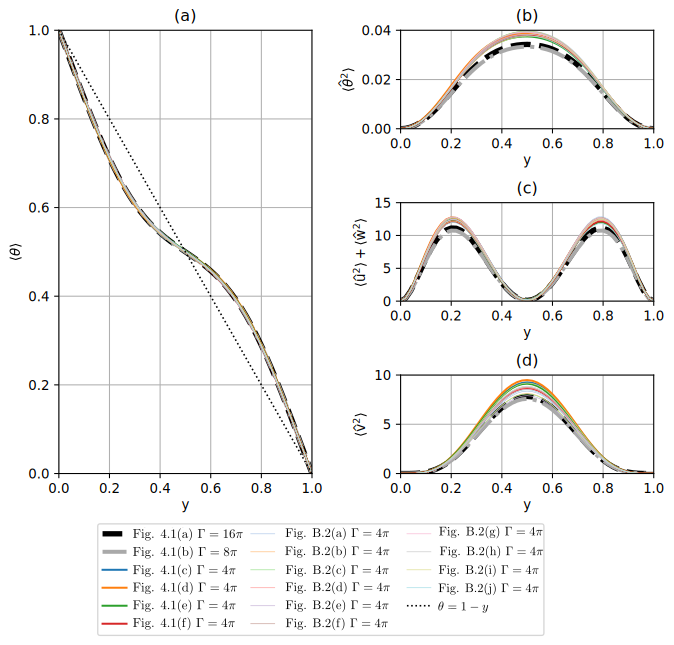
\includegraphics[width=0.8\textwidth]{StateSpaceStructureOfSDC/Figures/wallNormStats.pdf} 
    \caption{Profiles of (a) averaged temperature, (b) root-mean-squared temperature fluctuation, (c) sum of root-mean-squared $x$-$z$ velocity fluctuations and (d) root-mean-squared wall-normal velocity fluctuations for the SDC and elementary states shown in figures \ref{fig:fig1}(a-f) and in Appendix \ref{app:appB}. Note that $\langle \cdot \rangle = \frac{1}{TL_xL_z}\int_{t,x,z} \cdot \; \mathrm{d}t \mathrm{d}x \mathrm{d}z$ refers to the time and plane averaged operator, where $T$ was chosen to be sufficiently long to ensure temporal convergence.}
    \label{fig:averagedProfile}
\end{figure}

The comparison between the time-averaged mean temperature profile, mean-squared temperature fluctuations, and mean-squared velocity fluctuations of SDC (figures \ref{fig:fig1}(a,b)) and elementary states (figures \ref{fig:fig1}(c-f) and figure \ref{fig:10elementaries}) are presented in figure \ref{fig:averagedProfile}. In figure \ref{fig:averagedProfile}(c), we present the sum of mean-squared $x$- and $z$- velocity fluctuations due to horizontal isotropy. The mean temperature profiles of the elementary states closely match those of SDC (figure \ref{fig:averagedProfile}(a)). Notably, the mean-squared temperature and velocity fluctuations between SDC states (grey and black dashed curves) of figures \ref{fig:averagedProfile}(b-d) are similar. The mean-squared temperature and velocity fluctuations profiles of elementary states are comparable to those of SDC but are in general, slightly larger in magnitudes.

The spatial-temporal complexity of SDC reduces when the domain size is reduced from $\Gamma = 8\pi$ to $\Gamma = 4\pi$, i.e. less disordered spatial features. Reducing the domain from $\Gamma = 4\pi$ to $\Gamma = 2\pi$ led to transient SDC before stabilising into many elementary states. From the conventional view, especially made in the context of shear flow turbulence, this is unexpected as the chaotic state (i.e. turbulence) is commonly described as solution trajectories wandering around unstable invariant solutions \cite{kerswell2005, eckhardt2007, kawahara2012, graham21}. However, in this particular case observed in RBC, the chaotic state (i.e. SDC) is instead stabilised into stable invariant solutions (elementary states). Despite this distinguished feature of the state space, each of the elementary states is still seen to emerge in a spatially localised manner of SDC in an extended domain (figure \ref{fig:fig1}), and their spatially-averaged statistics are remarkably similar to those of SDC in extended domains (figure \ref{fig:averagedProfile}). Therefore, we consider the elementary states in the minimal domain to be the `building blocks' structure of SDC. 

%%%%%%%%%%%%%%%%%%%%%%%%%%%%%
% MULTIPLICITY OF EDGE STATES
%%%%%%%%%%%%%%%%%%%%%%%%%%%%%
\section{Multiplicity of edge states}\label{sec:rbc_edgestate}
The stable nature of many ISRs and elementary states underpinning SDC implies the existence of state-space boundaries between them (i.e. edge).
In this section, we perform the edge tracking between the stable manifolds of ISRs and elementary states to compute the attractors on the edge (i.e edge states). 
For the edge tracking, we use the bisection method \cite{skufca2006,Schneider2007, khapko_2016}, with an initial condition given by
\begin{equation}\label{eq:rbc_8}
    \mathbf{s_0}(\mathbf{x},t = 0) = \chi\mathbf{s}_{ISR,q} + (1 - \chi)\mathbf{s}_{elementary},
\end{equation}
where $\mathbf{s_0}(=[\mathbf{u}_0, \theta_0, p_0]^T)$ refers to an initial condition consisting of a weighted sum, $\chi \in [0,1] $, between a stable ISR state, $\mathbf{s}_{ISR,q}$ of a wavenumber $q$, and an elementary state, $\mathbf{s}_{elementary}$ where the subscript refers to its names in figures \ref{fig:fig1}(c-f).

Given the large number of stable ISRs and elementary states, we shall focus on the computation of the edge states considering three of the stable ISRs and two of the elementary states. However, in principle, the edge tracking is technically possible with other stable ISRs and elementary states. As such, in general, multiple edge states are expected. The three ISRs are related to three different wavenumbers, denoted by $\mathbf{s}_{ISR, q=2.06/d},  \mathbf{s}_{ISR,q=2.24/d}, \mathbf{s}_{ISR,q=3.16/d}$ (figures \ref{fig:ISRs}(b,d,j)) respectively, and the two elementary states are SD state, $\mathbf{s}_{spiral-defect}$ (figure \ref{fig:fig1}(c)), and PM state, $\mathbf{s}_{pacman}$ (figure \ref{fig:fig1}(d)). Using this set of stable ISRs and elementary states, we aim to track the edge near $\mathbf{s}_{ISR,q}$ in the direction of $\mathbf{s}_{elementary}$ by bisecting the initial condition with $\chi$ in (\ref{eq:rbc_8}), whereby one of the two trajectories across the edge decays toward $\mathbf{s}_{ISR,q}$ and the other is attracted toward transient chaotic state (i.e. SDC), referred to as the `lower' and `upper' trajectories respectively. The bisection of the initial condition is carried out by monitoring the difference in two trajectories with  $Nu$ (i.e. $\Delta Nu$). When the two trajectories reach a certain time at which $\Delta Nu > 0.0007$, the bisection of the initial condition is repeated using the flow fields from the two different trajectories by replacing $\mathbf{s}_{ISR,q}$ and $\mathbf{s}_{elementary}$ in (\ref{eq:rbc_8}) with them. This process is repeated until the edge trajectory reaches an attractor (i.e. an edge state).

\begin{figure}
    \centering
    \includegraphics[width=\textwidth]{StateSpaceStructureOfSDC/Figures/EdgeStatesSummary.pdf}
    \caption{Mid-plane termperature fields of ISRs and elementary states used in Eq. (\ref{eq:rbc_8}), and the resulting edge states. Here, ISRs (green borders): (a) $\mathbf{s}_{ISR, q=2.06/d}$, (b) $\mathbf{s}_{ISR,q=2.24/d}$, (c) $\mathbf{s}_{ISR,q=3.16/d}$; elementary states: (d) $\mathbf{s}_{pacman}$, (e) $\mathbf{s}_{spiral-defect}$; edge states (black borders): (f) $\emph{jagged}$, (g) \emph{point-defect}, (h) \emph{forked} and (i) \emph{skewed-varicose} edge state.}
    \label{fig:EdgeSummary}
\end{figure}

\begin{table}
    \centering
    \begin{tabular}{c|c|c|c}
        $\mathbf{s}_{ISR,q}$ & $\mathbf{s}_{elementary}$ & Edge state & State transitioned \\
        \hline
        $\mathbf{s}_{ISR,q=2.06/d}$ & $\mathbf{s}_{spiral-defect}$ & \emph{Jagged} (Stationary) & Transient Chaos \\
        $\mathbf{s}_{ISR,q=2.06/d}$ & $\mathbf{s}_{pacman}$ & \emph{Jagged} (Stationary) & Transient Chaos \\
        $\mathbf{s}_{ISR,q=2.24/d}$ & $\mathbf{s}_{spiral-defect}$ & \emph{Point-defect} (Travelling wave)  & $\mathbf{s}_{bubble-defect}$ \\
        $\mathbf{s}_{ISR,q=2.24/d}$ & $\mathbf{s}_{pacman}$ & \emph{Forked} (Relative Periodic Orbit)  & Transient Chaos \\
        $\mathbf{s}_{ISR,q=3.16/d}$ & $\mathbf{s}_{spiral-defect}$ & \emph{Skewed-varicose} (Stationary) & Transient Chaos \\
        $\mathbf{s}_{ISR,q=3.16/d}$ & $\mathbf{s}_{pacman}$ & \emph{Skewed-varicose} (Stationary) & Transient Chaos \\

    \end{tabular}
    \caption{A summary of the edge states computed. The first two columns denote the pair of initial conditions considered for edge tracking in Eq. (\ref{eq:rbc_8}). The names and classification of the edge states are described in the third column. The last column describes the state transitioned from $\mathbf{s}_{ISR,q}$ for sufficiently large $\chi$ in Eq. (\ref{eq:rbc_8}).}
    \label{tab:EdgeSummary}
\end{table}

Table \ref{tab:EdgeSummary} summarises the edge states and their dynamical properties computed from six combinations of $\mathbf{s}_{ISR,q}$ and $\mathbf{s}_{elementary}$ states, and they are visualised with the mid-plane temperature field in figure \ref{fig:EdgeSummary}.
The convection patterns of edge states are often featured with  mild spatial complexity compared to SDC and the elementary states.
In particular, their patterns contain the underlying convection pattern of $\mathbf{s}_{ISR,q}$ with spatially localised defects.
We obtained four edge states: specifically, the \emph{jagged} and \emph{skewed-varicose} edge states are stationary, and the \emph{point-defect} and \emph{forked} edge states are travelling wave and a relative periodic orbit respectively.
The \emph{jagged}, \emph{skewed-varicose} and \emph{forked} edge states lie on the boundary, separating the basins of attraction of stable $\mathbf{s}_{ISR,q}$ from transient SDC. In the case of the \emph{point-defect} edge state, the solution trajectory is found to bypass the transient SDC state, directly settling into a stable elementary state characterised by bubble-like convection roll defects, $\mathbf{s}_{bubble-defect}$.
Since the \emph{jagged}, \emph{skewed-varicose}, \emph{forked} edge states are similar in nature, acting as separatrices between $\mathbf{s}_{ISR,q}$ states and transient SDC, we will focus our analysis on the \emph{jagged} edge state only, alongside the \emph{point-defect} edge state.

\begin{figure}
\centering
\includegraphics[width=\textwidth]{StateSpaceStructureOfSDC/Figures/ISR2.06-SpiralDefect-EdgeTrajectory.pdf}
\caption{(a) Time history of $Nu$ and (b-e) the corresponding mid-plane temperature field snapshots at $t=2.0,6.5,31.0,65.5$ along the edge trajectory obtained by bisecting $\mathbf{s}_{ISR,q=2.06/d}$ and $\mathbf{s}_{spiral-defect}$.}
\label{fig:JaggedEdgeTrajectory}
\end{figure}

Using $Nu$ as an observable, successive bisections between $\mathbf{s}_{ISR, q = 2.06/d}$ and $\mathbf{s}_{spiral-defect}$ reveal the trajectory along the edge, as illustrated in figure \ref{fig:JaggedEdgeTrajectory}.
The trajectory along the edge spans from $t \approx 0 - 15$, and is initially characterised by a `speckled' defect (figure \ref{fig:JaggedEdgeTrajectory}(b)).
The `speckled' defect grows into a spatially localised jagged-liked defect as the trajectory is attracted to the \emph{jagged} stationary edge state from $t \approx 6.5$ onwards (figures \ref{fig:JaggedEdgeTrajectory}(c-e)).
We further examine the two trajectories in the opposite directions along the unstable manifold of the \emph{jagged} edge state in figure \ref{fig:ISR2.06-SpiralDefect-TwoTraj}, where the `upper' trajectory evolves into a transient SDC and the `lower' trajectory decays into the original stable $\mathbf{s}_{ISR,q=2.06/d}$ state.
Starting from the `upper' trajectory (figure \ref{fig:ISR2.06-SpiralDefect-TwoTraj}(a)), the spatially localised jagged defect grew in the direction normal to the roll orientation at $t = 80.5$ (figure \ref{fig:ISR2.06-SpiralDefect-TwoTraj}(b)), contaminating the adjacent roll structure and propagating through the domain where transient SDC emerges from $t > 80.5$, lasting up to $t \approx 120$ (a snapshot of transient chaotic SDC regime at $t = 90.5$ is shown in figure \ref{fig:ISR2.06-SpiralDefect-TwoTraj}(c)).
The trajectory subsequently stabilises into a travelling-wave PM elementary state described by `pac-man' like patterns, propagating along the $-x$ direction from $t=125.5$ to $t=170.5$ (figures \ref{fig:ISR2.06-SpiralDefect-TwoTraj}(d,e)).
This is reminiscent of a secondary cross-roll instabilities experienced by low-wavenumber ISRs (such as $\mathbf{s}_{ISR,q=2.06/d}$ considered here), where a defect propagates in the direction perpendicular to the rolls \cite{bodenschatz2000}.
Along the `lower' trajectory (figure \ref{fig:ISR2.06-SpiralDefect-TwoTraj}(f)), the jagged defects diffuses from $t = 70.5$ to $t=75.5$, decaying into the stable $\mathbf{s}_{ISR,q=2.06/d}$ state at $t = 80.5$ (figures \ref{fig:ISR2.06-SpiralDefect-TwoTraj}(g-j)).


\begin{figure}
\centering
\includegraphics[width=\textwidth]{StateSpaceStructureOfSDC/Figures/ISR2.06-SpiralDefect-TwoTrajectories.pdf}
\caption{Time history of $Nu$ along two opposite directions along the unstable manifold of the \emph{jagged} edge state: (a) `upper' trajectory leading to a transient SDC for $t \approx 85 - 120$ and subsequently to PM state for $t>120$ and (f) `lower' trajectory stabilising into $\mathbf{s}_{ISR,q=2.06/d}$. Mid-plane temperature fields are visualised in (b-e) along the upper trajectory at $t = 80.5,~90.5,~125.5,~170.5$, and in (g-j) along the lower trajectory at $t = 70.5, 75.5, 80.5, 85.5$.}
\label{fig:ISR2.06-SpiralDefect-TwoTraj}
\end{figure}


\begin{figure}
\centering
\includegraphics[width=\textwidth]{StateSpaceStructureOfSDC/Figures/ISR2.24-SpiralDefect-EdgeTrajectory.pdf}
\caption{a) Time history of $Nu$ and (b-e) the corresponding mid-plane temperature field snapshots at $t=4,13,22.5,40.5$ along the edge trajectory obtained by bisecting $\mathbf{s}_{ISR,q=2.24}$ and $\mathbf{s}_{spiral-defect}$.}
\label{fig:PointDefectEdge}
\end{figure}

\begin{figure}
\centering
\includegraphics[width=\textwidth]{StateSpaceStructureOfSDC/Figures/ISR2.24-SpiralDefect-TwoTrajectories.pdf}
\caption{Time history of $Nu$ along two opposite directions of the unstable manifold of the \emph{point-defect} edge state: (a) `upper' trajectory leading a stationary elementary state with bubble defect from $t \approx 43 - 163$ and (f) `lower' trajectory decaying to the stable $\mathbf{s}_{ISR,q=2.24}$ state. Mid-plane temperature fields are visualised in (b-e) along the upper trajectory at $t = 43.0, 58.0, 83.0, 163.0$, and in (g-j) along the lower trajectory at $t = 38.0, 43.5, 44.5, 53.0$.}
\label{fig:ISR2.24-SpiralDefect-TwoTraj}
\end{figure}

Next, we analyse the edge trajectory obtained bisecting between $\mathbf{s}_{spiral-defect}$ and $\mathbf{s}_{ISR,q=2.24}$ in figure \ref{fig:PointDefectEdge}.
The trajectory along the edge from $t = 4$ (figure \ref{fig:PointDefectEdge}(b)) is described by time-dependent convection structures.
The edge trajectory began to be stabilised into the \emph{point-defect} edge state from $t = 13$ onwards (figure \ref{fig:PointDefectEdge}(c)), propagating along $x$ direction from $t=22.5$ (figures \ref{fig:PointDefectEdge}(d,e)).
It is characterised by the convection structure of the $\mathbf{s}_{ISR,q=2.24}$ state with a pointed defect structure, hence referred to as the \emph{point-defect} edge state.
The upper and lower trajectories through two opposite directions of the unstable manifold of the travelling wave \emph{point-defect} edge state are subsequently examined in figure \ref{fig:ISR2.24-SpiralDefect-TwoTraj}.
Integrating along the upper trajectory (figure \ref{fig:ISR2.24-SpiralDefect-TwoTraj}(a)), the spatially localised point-defect structure grew from $t = 43$ to $t= 83$ (figures \ref{fig:ISR2.24-SpiralDefect-TwoTraj}(b-d)), saturating into a stationary elementary state at $t=163$ (figure \ref{fig:ISR2.24-SpiralDefect-TwoTraj}(e)) characterised by $\mathbf{s}_{ISR,q=2.24}$ with a large bubble defect.
Along the lower trajectory (figure \ref{fig:ISR2.24-SpiralDefect-TwoTraj}(f)), the spatially localised point defect merged onto the adjacent convection roll from $t=38$ to $t=44.5$ (figures \ref{fig:ISR2.24-SpiralDefect-TwoTraj}(g,h,i)), stabilising into the $\mathbf{s}_{ISR,q=2.24/d}$ state at $t = 53$  (figure \ref{fig:ISR2.24-SpiralDefect-TwoTraj}(j)). 
It is worth noting that, in this particular case, no chaotic transient in the form of SDC has been observed.

\begin{figure}
    \centering
    \includegraphics[width=0.9\linewidth]{StateSpaceStructureOfSDC/Figures/PhaseSpace-ISR-Elem-SDC-Edges-Bands.pdf}
    \caption{Phase portrait of the \emph{jagged}, \emph{point-defect}, \emph{defect} and \emph{skewed-varicose} edge states, along with stable ISRs, elementary states and transient SDC. Green and grey horseshoe lines are the regions, where stable ISRs and edge attractors are expected to be distributed when different sizes of the computational domain are considered.}
    \label{fig:statespace-sdc-isr-elems-edge}
\end{figure}

Finally, figure \ref{fig:statespace-sdc-isr-elems-edge} depicts a state space portrait of stable ISRs, SDC and the edge/elementary states found here. As seen previously, SDC and elementary states are seen to be clustered around the region of $||\frac{1}{\overline{V}}\tilde{\mathbf{u}}||_2\approx 6.3$ and $||\frac{1}{\overline{V}}RaPr\tilde{\theta}||_2\approx 8.6$, whereas stable ISRs are distributed along a horseshoe-shaped band (green line). The edge states found in this study are located not far from the (green) horseshoe-shaped band of ISRs, as they presumably lie in a smaller (grey) horseshoe-shape band situated between ISRs and SDC or elementary states. While we have identified four edge states, we expect that there are more edge states, presumably distrubuted along the (grey) horseshoe-shaped band. It is also worth mentioning that the edge states we found here contain the underlying ISR structure ($\mathbf{s}_{q=2.06/d,2.24/d,3.16/d}$) modified by spatially localised defects and `pinches' between rolls, supporting its proximity with ISRs in the state space. This feature is also reminiscent of spatially localised edge states identified in boundary layer flows \cite{khapko_2016}. Lastly, we would like to emphasise that we have only considered initial conditions from the states between $\mathbf{s}_{ISR,q}$ and $\mathbf{s}_{elementary}$ and not strictly between $\mathbf{s}_{ISR,q}$ and a transient SDC state. Nevertheless, three of the edge states are found to lie on the boundary separating the stable ISRs from transient SDC, supporting previous findings that the transient chaotic SDC are related to elementary states.

\section{Unstable ideal straight rolls}\label{sec:rbc_asymp}
Thus far, we have studied the edge and the edge states between some of the stable ISRs and elementary states. The dynamics associated with the unstable ISRs outside of the Busse balloon, however, remain unclear \cite{busse1985}. Given that the stable ISRs and SDC form a bistable system, it is expected that some of the unstable ISRs near the Busse balloon would asymptotically reach one of the stable ISRs as the difference between the stable and unstable ISRs would be sufficiently small \cite{steinberg1985,croquette1989a}. On the other hand, the unstable ISRs, which exist far from the boundary of the Busse balloon, may well have a sufficiently large deviation from the stable ISRs, implying that they are possibly associated with a state-space route to the SDC. The purpose of this section is to test this hypothesis by examining the long-term behaviour of the linear instabilities of the unstable ISRs.

We consider the linear instabilities of 3 unstable ISRs on the right side of the Busse balloon, with increasing wavenumber of $q=3.5/d, 4.0/d, 4.5/d$, as shown in figure \ref{fig:bbfig}(a). The identification of the linear instability mode (or unstable manifold) with the different spanwise wavenumbers $\beta$ is considered (see \eqref{eq:rbc_simAnsatz}). Figure \ref{fig:bbfig}(b) presents the unstable eigenvalues as a function of $\beta$. There are 2, 4 and 7 unstable manifolds ($\Re (\lambda) > 0$) for unstable ISRs of $q = 3.5/d, 4.0/d, 4.5/d$ respectively, forming total 13 unstable manifolds. In general, the growth rate and the number of linear instability modes (i.e. the repelling strength and the number of unstable manifolds) increase as $q$ increases. It is worth mentioning that the solutions of unstable ISRs of $\mathbf{s}_{ISR,q}(x,y)$ (required for linear stability analysis) are obtained by restricting the computational domain to the 2D $x$-$y$ plane which artificially suppresses 3D linear instabilities. We also note that the stability analysis of the unstable ISR, $q = 5.0/d$ was not considered as it quickly evolved into an unstable ISR of $q = 3.5/d$, which will be discussed in section \S\ref{sec:rbc_heteroclinic}.

\begin{figure}
    \centering
    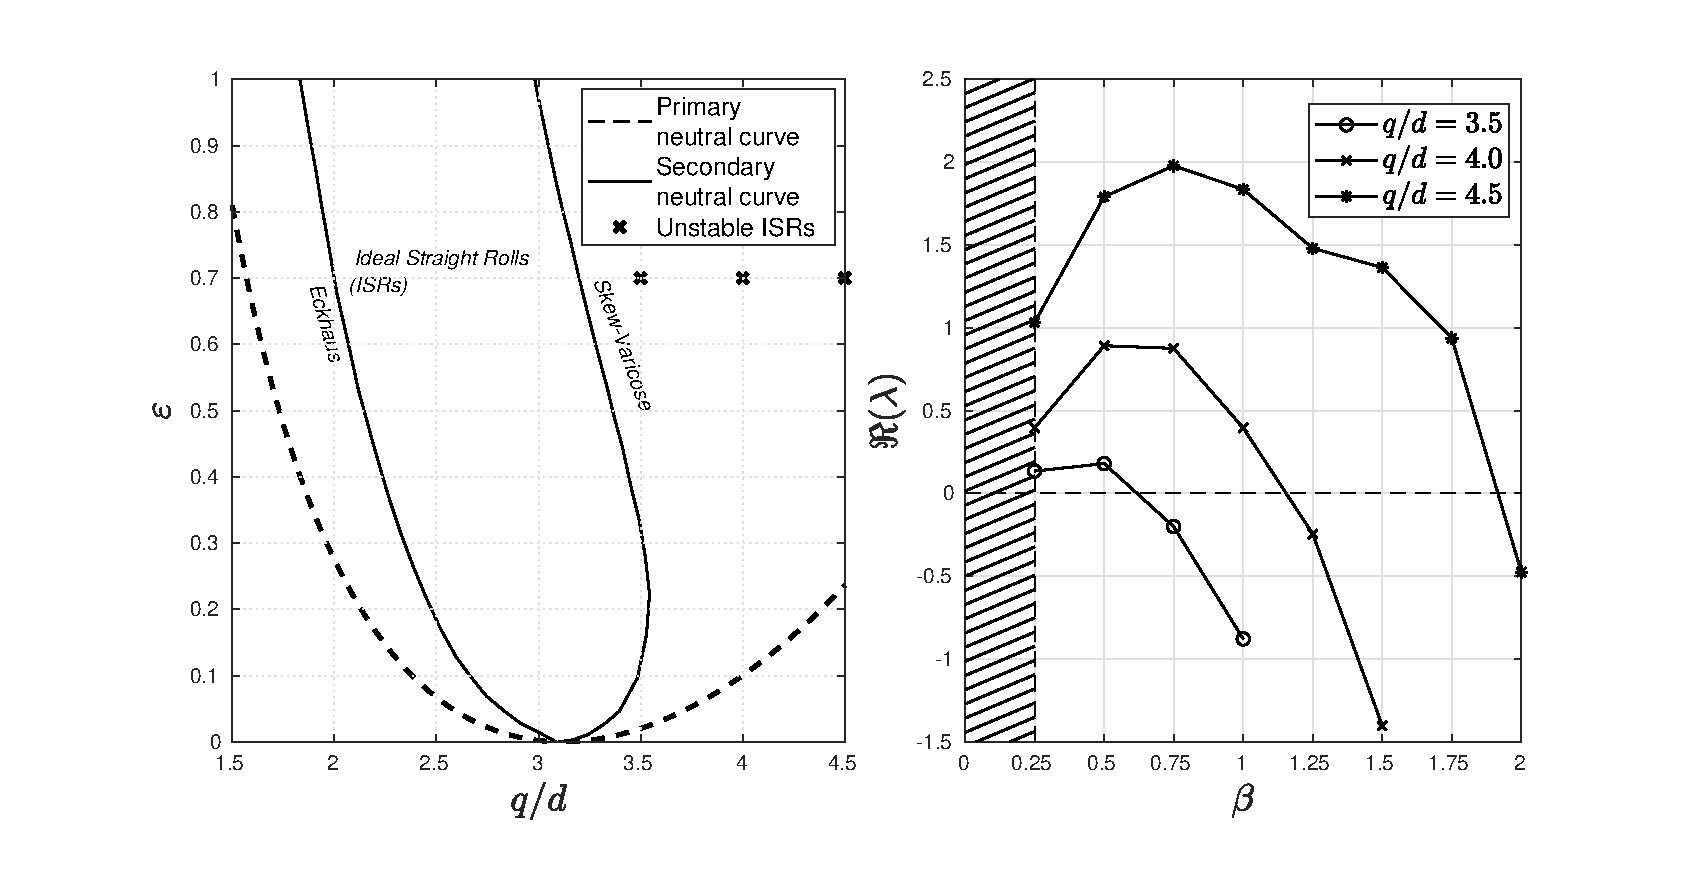
\includegraphics[width=\textwidth]{StateSpaceStructureOfSDC/Figures/bbfig.eps}
    \caption{(a) Primary and secondary (Busse balloon from figure 1 \cite{Decker94}) stability curves and unstable ISRs with $q = 3.5/d, \, 4.0/d, 4.5/d$; (b) Variation of the growth rate of instabilities of unstable ISRs as a function of spanwise wavenumber $\beta$. (Note that there are a total 13 unstable eigenmodes.)}
    \label{fig:bbfig}
\end{figure}

\begin{table}
\centering
\scalebox{0.88}{
\begin{tabular}{c | c c c c c c c}
     Cases & $\beta = 0.25$ & $\beta = 0.50$ & $\beta = 0.75$ & $\beta = 1.00$ & $\beta = 1.25$ & $\beta = 1.50$ & $\beta = 1.75$ \\
     \hline
     $q = 3.5/d$ & ISR$_{3.04}$ & (a) ISR$_{2.50}$ & Stable & Stable & Stable & Stable & Stable \\
     $q = 4.0/d$ & ISR$_{2.50}$ & (b) ISR$_{3.16}$ & ISR$_{3.00}$ & ISR$_{2.83}$ & Stable & Stable & Stable \\
     $q = 4.5/d$ & ISR$_{2.50}$ & ISR$_{2.50}$ & (c) ISR$_{3.00}$ & ISR$_{3.20}$ & (d) Elementary & ISR$_{2.50}$ & (e) Elementary 
\end{tabular}
}
\caption{Asymptotic state of secondary linear instabilities of $q = 3.5/d, 4.0/d, 4.5/d$. Subscripts in ISR refer to asymptotic wavenumber $q$, e.g., ISR$_{2.5}$ refers to ideal straight rolls with wavenumber of $q = 2.5/d$. The asymptotic behaviours of (a-c) and (d,e) are discussed further in \S\ref{sec:rbc_heteroclinic} and \S\ref{sec:rbc_chaoticsaddle} respectively.}
\label{tab:asymptotics}
\end{table}

To consider the long-term behavior in the direction of the unstable manifolds, an initial condition,
\begin{equation}\label{eq:rbc_SecInstab}
    \mathbf{s}_0(\mathbf{x},t=0) = \mathbf{s}_{ISR,q}(\mathbf{x}) + \mathbf{\hat{s}}_\beta(x,y)e^{i\beta z},
\end{equation}
is prescribed to equation \eqref{eq:rbc_rbc}. Here, $\hat{\mathbf{s}}_\beta e^{i\beta z}$ is the unstable eigenmode, the amplitude of which was scaled such that its total energy (defined in \eqref{eq:rbc_simAnsatz}) of $\delta = 10^{-5}, 10^{-4}, 10^{-3}$ were considered. The total energy of the eigenmode, $\delta = 10^{-4}$  was found to be sufficiently small enough to ensure linear growth, while large enough to prevent other eigenmodes from being excited. Next, the initial condition is time integrated over an extended period until an asymptotic state is reached. Table \ref{tab:asymptotics} shows the asymptotic states of $13$ linear instabilities, depicted in figure \ref{fig:bbfig}(b), of which 11 linear instabilities led to ISRs states, forming a network of heteroclinic orbits which will be discussed in \S\ref{sec:rbc_heteroclinic}. Only the remaining 2 instabilities led to a transient SDC state before settling into an elementary state discussed further in \S\ref{sec:rbc_chaoticsaddle}.

\begin{figure}
    \centering
    \includegraphics[width=\textwidth]{StateSpaceStructureOfSDC/Figures/phaseL2Plot-combined-wISRs-heteroclinicOrbits-combined.pdf}
    \caption{The phase-space solution trajectories connecting: (a) unstable base (conductive) state between 10 unstable rolls ($q = 5/d$), 7 unstable rolls ($q = 3.5/d$) and 5 stable rolls ($q = 2.5/d$); (b) unstable base (conductive) state between 8 unstable rolls ($q = 5/d$) and 6 stable rolls ($q = 3.16/d$); (c) unstable base (conductive) state between 9 unstable rolls ($q = 4.5/d$) and 6 stable rolls ($q = 3/d$). Here, the size of the arrows indicates the speed of the solution trajectory (or flow).}
    \label{fig:heteroclinics}
\end{figure}

%%%%%%%%%%%%%%%%%%%%%%%%%%%%%%%%%%%%%%%%%%%%
% Asymptotic behaviour -> Heteroclinic Orbit
%%%%%%%%%%%%%%%%%%%%%%%%%%%%%%%%%%%%%%%%%%%%
\subsection{Pathways leading to ISRs - heteroclinic orbits}\label{sec:rbc_heteroclinic}
In this section, the asymptotic behaviour of the most unstable linear instabilities of ISRs (tab \ref{tab:asymptotics}(a-c)) will be discussed. 
Figure \ref{fig:heteroclinics} depicts the state space plot of volume normalised L2-norms of velocity and temperature. It reveals a number of heteroclinic orbits, connecting the base state ($\bullet$), stable ($\color{green}{\bullet}$) and unstable ($\color{red}{\bullet}$) ISRs. Figure \ref{fig:heteroclinics}(a) exhibits several solution trajectories linking the base state, stable and unstable ISRs: three orbits connecting the base state to all the stable and unstable ISRs shown, one from the ISR of $q = 3.5/d$ to that of $q = 2.5/d$, and one from the ISR of $q = 5.0/d$ to that of $q = 3.5/d$. Here, caution will need to be taken in interpreting each of the connections as a heteroclinic orbit, because there appears to be an invariant state at which the speed of the solution trajectory nearly vanishes (a sign of the existence of unstable invariant states or ghost states \cite{strogatz_2018}): for example, see the solution trajectory between the ISR of $q = 3.5/d$ to that of $q = 2.5/d$ (in the inset of figure \ref{fig:heteroclinics}(a)), which will be discussed below with figure \ref{fig:7RollsBeta0.50}. Starting from the primary base state, the system saturates into an ISR of wavenumber $q = 5.0/d$. Since this ISR is linearly unstable, it evolves into another unstable ISR of $q = 3.5/d$, before ultimately stabilising into an ISR of $q = 2.5/d$.  Next, figure \ref{fig:heteroclinics}(b) shows three solution trajectories connecting the base state, an unstable and stable ISR. Starting from the base state, the system transitions into an unstable ISR of $q = 4/d$ before stabilising into an ISR of $q = 3.16/d$. 
Lastly, figure \ref{fig:heteroclinics}(c) presents three solution trajectories connecting the base state, a stable and unstable ISR. Starting from the base state, it can evolve to an unstable ISR of $q = 4.5/d$ before settling into a stable ISR of $q = 3.0/d$. 
Figure \ref{fig:heteroclinics} suggests that each of the stable ISRs within the Busse balloon has the basin of attraction, characterised by a web of heteroclinic orbits connecting some of the unstable ISRs outside of the Busse balloon. It is worth emphasising that the connections between the solutions presented here were obtained by time-integrating the dominant unstable manifolds of ISRs. In practice, there are many more unstable manifolds (see table \ref{tab:asymptotics}) which have not been presented, potentially leading to more complex networks of heteroclinic orbits that form the basin of attraction for each stable ISR.

Figure \ref{fig:7RollsBeta0.50} describes the asymptotic behaviour with the most unstable eigenmode for $q=3.5/d$ (table \ref{tab:asymptotics}(a)) in detail, corresponding to the connection between the unstable ISR of $q = 3.5/d$ and the stable ISR of $q = 2.5/d$ in figure \ref{fig:heteroclinics}(a). To observe the linear instability defined in Eq. (\ref{eq:rbc_SecInstab}), we report contribution of modal energy (figure \ref{fig:7RollsBeta0.50}(a)) as
\begin{equation}
    E_k(t) = \frac{1}{2} \int_\Omega |\hat{\mathbf{u}}_k(t)|^2 \; \mathrm{d}\Omega,
\end{equation}
where $\mathbf{\hat{u}}_k$ refers to the $k$-th Fourier coefficient in $z$-direction. Initially, the simulation starts from the ISR state of 7 rolls ($t = 33$), corresponding to a roll-wavenumber of $q = 3.5/d$. The unstable eigenmode $\mathbf{\hat{s}}_{\beta = 0.50}$ grows exponentially before peaking at $t=48.50$, forming an `S'-liked symmetric state (figure \ref{fig:7RollsBeta0.50}(c)). Note that, at this point, the time derivative of $E_k(t)$ nearly vanishes, indicating that the snapshot taken at $t=48.50$ is potentially close to an unstable invariant state. Finally, the modal energy of $N_z = 2$ decays and the system settles into an ISR state of $q = 2.5/d$ (5 rolls aligned in the x-direction), which is within the Busse balloon.

\begin{figure}
    \centering
    \includegraphics[width=0.9\textwidth]{StateSpaceStructureOfSDC/Figures/transitionPlot-7RollsBeta0.50.pdf}
    \caption{Asymptotic behaviour of the linear instability ($\hat{\mathbf{q}}_{\beta = 0.50}$) about unstable ISR $q = 3.5/d$. (a) Modal energy $E_k(t)$, and temperature snapshots, $\theta(x,z)|_{y=d/2}$ at (b) $t = 33$, (c) $t = 48.5$, (d) $t = 60$.}
    \label{fig:7RollsBeta0.50}
\end{figure}

Figure \ref{fig:8RollsBeta0.50} illustrates the asymptotic behaviour with the most unstable eigenmode for $q=4.0/d$ (table \ref{tab:asymptotics}{b}), also depicted in the solution trajectory connecting the unstable ISR of $q = 4.0/d$ to the stable ISR of $q = 3.16/d$ in figure \ref{fig:heteroclinics}(b). Figure \ref{fig:8RollsBeta0.50}(a) shows the contribution of modal energy from each Fourier $z$ component.
From $t=5-10$, the system experiences an exponential growth, guided by its dominant secondary eigenmode $\mathbf{\hat{s}}_{\beta=0.50}$, where the 8 rolls ISRs `disintegrates' into a convection pattern characterised by a symmetric `D' convection pattern.
Finally, the system stabilises into an ISR state with wavenumber $q = 3.16/d$.

\begin{figure}
    \centering
    \includegraphics[width=0.9\textwidth]{StateSpaceStructureOfSDC/Figures/transitionPlot-8RollsBeta0.50.pdf}
    \caption{Asymptotic behaviour along the linear instability $\hat{\mathbf{s}}_{\beta = 0.50}$ about unstable ISR $q=4.0/d$. (a) Modal energy $E_k(t)$, and temperature snapshots, $\theta(x,z)|_{y=d/2}$ at (b) $t = 5$, (c) $t = 10.5$, (d) $t = 12.5$.}
    \label{fig:8RollsBeta0.50}
\end{figure}

Figure \ref{fig:9RollsBeta0.75} presents the asymptotic behaviour with the most unstable eigenmode for $q=4.5$ (table \ref{tab:asymptotics}(c)), corresponding to the connection between the unstable ISR ($q=4.5/d$) and the stable ISR ($q = 3/d$) in figure \ref{fig:heteroclinics}(c). Figure \ref{fig:9RollsBeta0.75}(a) shows the contribution of modal energy from each Fourier $z$ component. Initially, the system begins as an ISR state of 9 rolls ($t = 1.25$). Next, the secondary eigenmode $\mathbf{\hat{s}}_{\beta = 0.75}$ grows exponentially and peaks at $t=4.50$, leading to an intermediate state characterised by a symmetric `O' convection rolls with small $d E_k(t)/dt$ (fig \ref{fig:9RollsBeta0.75}(c)). Finally, the system evolved into an ISR state of $q = 3/d$ as an asymptotic state.

All three cases examined here show that the transition from an unstable ISR to a stable ISR involves an intermediate state, at which $d E_k(t)/dt$ is seen to be relatively small. In the transition pathway from the unstable to stable ISR, it is presumable that there exists an unstable equilibrium (i.e. fixed point/travelling-waves etc.) in the form of the original unstable ISR with its nonlinearly saturated instability, or ghost states \cite{strogatz_2018}. The existence of such a stationary solution can probably be computed with a typical Newton iteration or variational methods \cite[]{Viswanath2007, Parker_2022}, but this is beyond the scope of the present study. In any case, the numerical experiments here suggest that each of the stable ISR has a basin of attraction composed of a network of heteroclinic orbits involving connections between the base state and unstable ISRs. 


\begin{figure}
    \centering
    \includegraphics[width=0.9\textwidth]{StateSpaceStructureOfSDC/Figures/transitionPlot-9RollsBeta0.75.pdf}
    \caption{Asymptotic behaviour along the linear instability of $\hat{\mathbf{s}}_{\beta = 0.75}$ about unstable ISR of $q=4.5/d$. (a) Modal energy $E_k(t)$, and temperature snapshots, $\theta(x,z)|_{y=d/2}$ at (b) $t = 1.25$, (c) $t = 4.50$, (d) $t = 8.75$.}
    \label{fig:9RollsBeta0.75}
\end{figure}
%%%%%%%%%%%%%%%%%%%%%%%%%%%%%%%
% PATHWAYS TO ELEMENTARY STATES
%%%%%%%%%%%%%%%%%%%%%%%%%%%%%%%
\subsection{Pathways leading to elementary states}\label{sec:rbc_chaoticsaddle}
Now, we discuss the asymptotic behaviour with linear instabilities of $\mathbf{\hat{s}}_{\beta=1.25}$ and $\mathbf{\hat{s}}_{\beta=1.75}$ about the unstable ISR of $q = 4.5/d$ (tab \ref{tab:asymptotics}(d,e)). Contrary to the transitions presented in the previous section, the asymptotic states did not result in ISRs, but transient SDC before settling into an elementary state for case (e) (table \ref{tab:asymptotics}(e)), and an elementary directly for case (d) (table \ref{tab:asymptotics}(d)).
\begin{figure}
    \centering
    \includegraphics[width=\textwidth]{StateSpaceStructureOfSDC/Figures/transitionPlot-9RollsBeta1.25-P4-dt0.01.pdf}
    \caption{Asymptotic behaviour along the unstable manifold of $q = 4.5/d, \beta = 1.25$. (a) Modal energy $E_k(t)$ plot, and temperature snapshots $\theta(x,z)|_{y=d/2}$ at (b) $t=1.25$, (c) $t = 5$, (d) $t = 6.75$, (e) $t = 8.75$, (f) $t=21.75$ and (g) $t = 25$}
    \label{fig:9rollsbeta1.25}
\end{figure}
The asymptotic behavior with $\mathbf{\hat{s}}_{\beta = 1.25}$ for unstable ISR $q = 4.5/d$ (table \ref{tab:asymptotics}(d)) is presented in figure \ref{fig:9rollsbeta1.25}. At $t=1.25$, the unstable ISR state ($q = 4.5/d$) is characterised by 9 rolls aligned along $x$ direction. Subsequently, the state experiences the linear instability triggered ($t=5$, figure \ref{fig:9rollsbeta1.25}(c)), shown as an exponential growth of the brown curve figure \ref{fig:9rollsbeta1.25}(a)), corresponding to the fifth Fourier modal energy (or $\beta = 1.25$). At $t=6.75$, the system transitions into a saturated state temporarily (albeit unstable), characterised by square-like alternating convection patterns (figure \ref{fig:9rollsbeta1.25}(d)), and saturates briefly at $t=8.75$, forming `S'-like convection patterns in figure \ref{fig:9rollsbeta1.25}(e). Finally, it settles into an oscillatory elementary state (i.e. stable periodic orbit) with an oscillation period of $T \approx 3.25$ (figures \ref{fig:9rollsbeta1.25}(f,g)).

The asymptotic behavior with $\mathbf{\hat{s}}_{\beta = 1.75}$ of unstable ISR $q = 4.5/d$ (table \ref{tab:asymptotics}(e)) is presented in figure \ref{fig:9RollsBeta1.75}. Starting from $t=1.25$, the unstable ISR state is characterised by 9 convection rolls aligned along the $x$-axis. The state experiences the linear instability imposed from $t=1.25$ to $t=7$, corresponding to an exponential growth in the grey curve ($E_7 (t)$ in figure \ref{fig:9RollsBeta1.75}(a)), marked by cross-convection rolls in figure \ref{fig:9RollsBeta1.75}(c). Subsequently, the state exhibits a transient SDC behaviour from $t \approx 7$ to $t \approx 80$, characterised by an `O'-ring and `pac-man' liked convection pattern illustrated in figure \ref{fig:9RollsBeta1.75}(d). Following this, the system stabilises into a short-period ($T \approx 1.8$) oscillatory behaviour between $t = 90$ and $t = 110$ (figure \ref{fig:9RollsBeta1.75}(e)),  before transitioning into a long-period time-periodic state from $t = 110$ to $t = 201.75$ (figure \ref{fig:9RollsBeta1.75}(a) $cont.$), with a period of $T = 51.75$. The convection pattern appears to be travelling diagonally in the negative $x$-$z$ directions (compare figures \ref{fig:9RollsBeta1.75}(f,g)), indicating that this state is a relative periodic orbit.  

Figure \ref{fig:phasespacetraj} presents the state space trajectories of two pathways discussed above, represented by the volume-normalised L2-norms of velocity perturbations, temperature perturbations and Nusselt number. These trajectories are superimposed upon the state space trajectories of SDC (figures \ref{fig:fig1}(a,b)), elementary states (figures \ref{fig:fig1}(c-f)) and the fixed-point attractors of ISRs (figure \ref{fig:statespace-sdc-isr-elems}). The purple trajectory represents the one along the linear instability direction (i.e. the unstable manifold) of $q=4.5/d$ with $\beta = 1.25$. Originating from the unstable ISR ($q = 4.5/d$), briefly saturates at $||\frac{1}{\overline{V}}\mathbf{\tilde{u}}|| \approx 6.25$ and $||\frac{1}{\overline{V}}RaPr\tilde{\theta}||_2 \approx 8$, before stabilising into a periodic orbit near the \emph{spiral-defect} elementary state (see figure \ref{fig:fig1}, represented by the orange trajectory in figure \ref{fig:statespace-sdc-isr-elems}. The case of $q = 4.5/d$ along the linear instability direction for $\beta = 1.75$ is represented by the brown trajectory. Emanating from the unstable ISR ($q = 4.5/d$), the trajectory experiences a period of transient SDC behaviour in the vicinity of elementary states before converging onto a relative periodic orbit, as expected from figure \ref{fig:9RollsBeta1.75}. It is evident that the two trajectories arising from linear instabilities about the unstable ISR ($q = 4.5/d$) lie within the vicinity of SDC.

\begin{figure}
    \centering
    \includegraphics[width=0.9\textwidth]{StateSpaceStructureOfSDC/Figures/transitionPlot-9RollsBeta1.75-P4-dt0.01.pdf}
    \caption{Asymptotic behaviour along the linear instability of $\hat{\mathbf{s}}_{\beta = 1.75}$ about unstable ISR $q = 4.5/d$. (a) Modal energy $E_k(t)$, and temperature snapshots $\theta(x,z)|_{y=d/2}$ at the onset of secondary instability at (b) $t = 1.25$, (c) $t=7$, following a transient SDC behaviour at (d) $t = 40$, and settling into a elementary state at (e) $t = 100$, (f) $t = 150$ and (g) $t = 201.75$.}
    \label{fig:9RollsBeta1.75}
\end{figure}
\begin{figure}
    \centering
    \includegraphics[width=0.8\textwidth]{StateSpaceStructureOfSDC/Figures/PhaseSpace-ISR-Elem-SDC-UnstblMnflds-arrows.pdf}
    \caption{State space visualisations using (a) $||\frac{1}{\overline{V}}\mathbf{\tilde{u}}||_2$ and $||\frac{1}{\overline{V}}RaPr\tilde{\theta}||_2$, for SDC shown in figure \ref{fig:fig1}(a,b), 4 elementary states shown in figures \ref{fig:fig1}(c-f), linear instabilities (purple) $\mathbf{\hat{s}}_{\beta=1.25}$, (brown) $\mathbf{\hat{s}}_{\beta=1.75}$ about an unstable ISR $q = 4.5/d$ (figures \ref{fig:9rollsbeta1.25}, \ref{fig:9RollsBeta1.75}), and stable fixed-points of ISRs for wavenumber $q \in (2.0/d, 3.35/d)$  with the magnitude of $q$ is depicted by the opacity of the filled symbol ($\color{green}{\bullet}$), with arrows denoting direction of increasing $q$. Figure (b) is a magnified plot of (a).}
    \label{fig:phasespacetraj}
\end{figure}

\subsection{A pathway to SDC in an extended domain $\Gamma = 4\pi$}\label{app:appC}

\begin{figure}
    \centering
    \includegraphics[width=\textwidth]{StateSpaceStructureOfSDC/Figures/transitionPlot-9RollsBeta1.75-P4-dt0.01-extendedDomain.pdf}
    \caption{Asymptotic behaviour along the linear instability $\hat{\mathbf{s}}_{\beta = 1.75}$ about unstable ISR $q = 4.50/d$, in an extended domain $\Gamma = 4\pi$. (a) Modal energy $E_k(t)$, and temperature snapshots $\theta(x,z)|_{y=d/2}$, at (b) $t = 1.25$, (c) $t = 7$, (d) $t = 40$, (e) $t = 100$, (f) $t = 125$, (g) $t = 150$.}
    \label{fig:extendeddomain}
\end{figure}

In \S\ref{sec:rbc_chaoticsaddle}, we have identified two distinct pathways to elementary states along some unstable manifolds from an unstable ISR. In particular, one of the trajectories evolved into transient SDC before stabilising into an elementary state. This is reminiscent of a chaotic saddle, but with a considerably short lifetime. The transient SDC behaviour observed within the minimal domain implies that if the same initial condition is added in an extended computational domain, it would trigger a chaotic state at least with a longer lifetime. This chaotic state is expected to be SDC in an extended domain, given the analysis in \S\ref{sec:rbc_chaoticsaddle}. To examine this hypothesis, we conduct a numerical simulation with an initial condition from the case of table \ref{tab:asymptotics}(e) (i.e. the unstable ISR $q = 4.5/d$ with the instability mode of $\mathbf{\hat{s}}_{\beta = 1.75}$) in a domain twice larger than each horizontal direction ($\Gamma = 12.58$). 

The solution trajectory along the unstable manifold, $\mathbf{s}_{\beta = 1.75}$, of ISR $q = 4.5/d$ in an extended domain ($\Gamma = 4\pi$) is presented in figure \ref{fig:extendeddomain}. The state, characterised by 18 convection rolls (figure \ref{fig:extendeddomain}(b)), experiences the linear instability from $t=1.25$ to $t=7$, marked by cross-convection rolls shown in figure \ref{fig:extendeddomain}(c). Subsequently, the state exhibits a prolonged period of chaotic behaviour, starting from $t=7$ and lasting beyond $t=200$. This is in stark contrast to the transient SDC behaviour observed in the minimal domain (figure \ref{fig:9RollsBeta1.75}), confirming the hypothesis above. Finally, it is interesting to note that the convection patterns of figures \ref{fig:extendeddomain}(f,g) contain localised structures that bear resemblance with the stationary \emph{pac-man} (figure \ref{fig:fig1})(c)) and oscillatory \emph{peanut} (figure \ref{fig:fig1}(f))  elementary states.


\begin{figure}
    \centering
    \includegraphics[width=\textwidth]{StateSpaceStructureOfSDC/Figures/statespace-compiled.pdf}
    \caption{State space sketch containing the base, stable and unstable ISRs, edge, elementary states and SDC in a confined domain. Open circles, ($\circ$) and filled circles/squares ($\bullet$, $\blacksquare$) refer to unstable and stable states. Solid ($-$) and dashed lines ($--$) are the solution trajectories along the primary and secondary instabilities respectively, $\lambda_{max}^{Pri,Sec}$ refers to the most unstable primary and secondary linear instability manifolds. Blue, orange and green trajectories denote heteroclinic connections leading toward stable ISRs (trajectories labelled (A-G) and colors adapted from figure \ref{fig:heteroclinics}). Dashed-dotted trajectories ($-\cdot-$) refer to solution trajectories emerging from the edge states (color-coded from figure \ref{fig:statespace-sdc-isr-elems-edge}). The dotted line ($\cdots$) represents the boundary between ISRs and SDC, consisting of many stable elementary states.}
    \label{fig:statespacesketch}
\end{figure}

%%%%%%%%%%%%%%%%%%%%%%%%%%%%%
% CONCLUSIONS AND FUTURE WORK
%%%%%%%%%%%%%%%%%%%%%%%%%%%%%
\section{Concluding remarks}\label{sec:rbc_4}
SDC has been considered one of the bistable states within a large spatial domain in Rayleigh-B\'{e}nard convection. However, existing studies have also shown the presence of multiple stable states in small and large domains, puzzling one's understanding of the bistable system in an extended spatial domain. 
Starting with numerical simulation in an extended domain ($\Gamma=8\pi$), we have systematically reduced the computational domain, such that the fundamental patterns of SDC can be isolated. 
Through numerical experiments confined within a minimal domain of $\Gamma = 2\pi$, we have identified transient SDC before stabilising into a stable elementary states of SDC, and 14 different elementary states have been found in this way.
From the conventional view of turbulence in shear flow, chaotic trajectories (representing turbulence) are expected to visit a set of unstable invariant solutions before eventually decaying to the base (laminar) state. However, in contrast to this expectation, the solution trajectory, once tangled into SDC stabilises into an non-trivial elementary state instead of returning to the base (ISR) state \cite{skufca2006, Lustro_2019}. This finding is new and challenges the understanding of transition from a dynamical system viewpoint.
Despite this, the elementary states are still situated around the chaotic trajectories of SDC in the state space (figure \ref{fig:statespace-sdc-isr-elems}), and their statistical properties (figure \ref{fig:averagedProfile}) are remarkably similar to those of SDC.
This suggests that the computed elementary states may serve as `building block' structures of SDC that interact with each other to form SDC in an extended domain.

To further understand the state space structure of SDC, ISRs and possible gateways toward SDC, we furnish a state space sketch of the solution trajectories connecting the base, stable and unstable ISRs, edge, elementary states and SDC, shown in figure \ref{fig:statespacesketch}.
Starting from the base state, time-integrating along the unstable manifold guided by primary instabilities leads to either stable or unstable ISRs, denoted by solid trajectories.
Notably, the most unstable primary instability leads to a 7 roll ISR ($q = 3.5/d$), before saturating into a stable 5 roll ISR ($q = 2.5/d$), following the most unstable secondary instability, depicted by dashed trajectories.
These solution trajectories form a network of heteroclinic orbits, connecting the base state with stable ($q = 2.5/d$) and unstable ($q = 3.5/d, 5/d$) ISRs, represented in blue.
Further from the boundaries of the Busse balloon, we have identified two more heteroclinic orbits that form a basin of attractor between the base state, and stable, unstable ISRs, labelled as a group of orange and green trajectories.
These heteroclinic orbits are expected in experimental settings where initial conditions and background noise can be controlled precisely.
In practice, where precise controls are inaccessible, it is more likely to observe SDC ($\Gamma = 4\pi ,8\pi$) or stable elementary states ($\Gamma = 2\pi$), which are embedded in the chaotic trajectories of SDC (see coloured $\blacksquare$), supporting the notion that SDC is underpinned by elementary states presumably interacting with each other.
By examining the edge states between stable ISRs and elementary states, we have identified 4 edge states that lie on the boundary between stable ISRs and transient SDC, where the upper and lower trajectories emerging from their unstable manifold are represented by dash-dotted trajectories.
Further from the Busse balloon, we have identified an unstable manifold of a 9 roll ($q=4.5/d$) ISR, leading to the onset of SDC. 
Consequently, the unstable base state is also expected to lie on the boundary, as a controlled initial condition could guide the system toward the unstable 9-roll ISR, and subsequently the onset of SDC.
Finally, the dotted line represents the boundary between ISRs and SDC, consisting of the base state, edge states and unstable 9 roll ISR ($q=4.5/d$), illustrating four possible routes toward SDC.
Although we have considered the unstable manifolds of ISRs for $\Gamma = 2\pi$, we acknowledge that the dimension of such manifolds depends on the domain size and that the presence of spatially subharmonic instabilities may arise as the domain size increases.
Additionally, there may well be other unstable ISRs and edge states along the boundary. However, the investigation into the existence of such states is challenging due to the daunting computational efforts required. Recent advances, such as the framework proposed in \cite{schmid2017}, may help to accelerate linear stability analysis and facilitate further investigations.
